\documentclass[conference]{IEEEtran}
\IEEEoverridecommandlockouts

\usepackage{cite}
\usepackage{amsmath,amssymb,amsfonts}
\usepackage{algorithmic}
\usepackage{graphicx}
\usepackage{textcomp}
\usepackage{xcolor}
\usepackage{iftex}
\usepackage{url}
\usepackage{placeins}
\usepackage{array}
\usepackage{multirow}
\ifXeTeX
\usepackage{fontspec}
\setmainfont{Times New Roman}
\setsansfont{Times New Roman}
\setmonofont{Times New Roman}
\else
\usepackage{newtxtext,newtxmath}
\renewcommand{\ttdefault}{\rmdefault}
\fi
\urlstyle{same}

\def\BibTeX{{\rm B\kern-.05em{\sc i\kern-.025em b}\kern-.08em
    T\kern-.1667em\lower.7ex\hbox{E}\kern-.125emX}}

\begin{document}

\title{Enhancing Brute Force Attack Detection in NIDS: A Hybrid Sampling and Ensemble Learning Approach}

\author{
\makebox[\textwidth][c]{%
\begin{minipage}[t]{0.30\textwidth}
\centering
{\normalsize Edward Aria Tanujaya}\\
{\itshape Computer Science Department,}\\
{\itshape School of Computer Science}\\
Bina Nusantara University\\
Jakarta, Indonesia 11480\\
edward.tanujaya001@binus.ac.id
\end{minipage}\hfill
\begin{minipage}[t]{0.30\textwidth}
\centering
{\normalsize Andrian Pratama}\\
{\itshape Computer Science Department,}\\
{\itshape School of Computer Science}\\
Bina Nusantara University\\
Jakarta, Indonesia 11480\\
andrian.pratama@binus.ac.id
\end{minipage}\hfill
\begin{minipage}[t]{0.30\textwidth}
\centering
{\normalsize Jeta Sunanda}\\
{\itshape Computer Science Department,}\\
{\itshape School of Computer Science}\\
Bina Nusantara University\\
Jakarta, Indonesia 11480\\
jeta.sunanda@binus.ac.id
\end{minipage}%
}\\[1em]
\makebox[\textwidth][c]{%
\begin{minipage}[t]{0.30\textwidth}
\centering
{\normalsize Hidayaturrahman}\\
{\itshape Computer Science Department}\\
{\itshape School of Computer Science}\\
Bina Nusantara University\\
Jakarta, Indonesia 11480\\
hidayaturrahman@binus.ac.id
\end{minipage}\hspace{0.06\textwidth}
\begin{minipage}[t]{0.30\textwidth}
\centering
{\normalsize Satriadi Putra Santika}\\
{\itshape Computer Science Department}\\
{\itshape School of Computer Science}\\
Bina Nusantara University\\
Jakarta, Indonesia 11480\\
satriadi.santika@binus.ac.id
\end{minipage}%
}
}

\maketitle

\begin{abstract}
Machine-learning-based Network Intrusion Detection Systems (NIDS) are widely used to detect malicious traffic, but their performance can degrade when attack classes are underrepresented. Previous studies have attempted to mitigate this through feature selection, sampling, and ensemble learning. However, this components are often failing to adequately address minority attacks. In dataset like CICIDS2017, Brute Force traffic remains difficult to detect because repeated authentication attempts closely resemble benign activity. This study focuses on Brute Force detection in the imbalanced CICIDS2017 dataset using a hybrid sampling and ensemble-learning pipeline. The proposed workflow maps CICIDS2017 labels into eight multiclass categories, limits the dominant Benign class, cleans invalid records, performs train-only feature selection using ANOVA \textit{SelectKBest} and correlation pruning, and applies SMOTE-Tomek only to the training partition. Two heterogeneous ensembles, soft voting and stacking, are then evaluated on an unseen test set. SMOTE-Tomek increased Brute Force training representation from 5,204 to 76,385 samples and reduced its imbalance ratio from 30.30:1 to 2.06:1. On the test set, soft voting achieved 98.73\% Brute Force precision, 92.78\% recall, and 95.66\% F1-score, while stacking achieved 98.28\% precision, 93.16\% recall, and 95.65\% F1-score. The results show that hybrid sampling and ensemble learning provide a practical strategy for Brute Force detection, although generalization beyond CICIDS2017 remains limited.
\end{abstract}

\begin{IEEEkeywords}
Network Intrusion Detection System, Brute Force Detection, CICIDS2017, SMOTE-Tomek, Ensemble Learning
\end{IEEEkeywords}

% ============================================================
\section{Introduction}
% ============================================================

Internet-based communication is now central to file sharing, remote access, and daily computing, but the same connectivity also expands the attack surface for private and organizational data. Recent threat reports show that cyberattacks continue to grow in both volume and stealth: malware-free detections increased from 62\% in 2021 to 71\% in 2022, while 75\% of attacks used to gain initial access were malware-free in 2023.\footnote{CrowdStrike Global Threat Reports, 2023 and 2024.} This trend shows that network defense requires detection mechanisms that can recognize suspicious behavior beyond known malware signatures.

Intrusion Detection Systems (IDS) are security mechanisms that monitor system or network activity and generate alerts when malicious behavior is detected \cite{singh2022minority}. IDS can be categorized into Host-based IDS (HIDS) and Network-based IDS (NIDS). HIDS monitors host-level information such as logs and resource usage, while NIDS observes network traffic flows. In this study, NIDS is selected because network-flow monitoring is suitable for detecting attack behavior across communication traffic and can be managed more centrally than host-by-host monitoring \cite{almuhanna2025anomaly,irfaissurur2025web}.

As network data continues to grow, traditional IDS approaches face difficulty in recognizing new or changing attack behavior. Machine learning and deep learning have therefore been used to improve NIDS because they can learn patterns from traffic data rather than relying only on fixed signatures \cite{almuhanna2025anomaly,ahmed2024explainable}. However, ML-based NIDS still has important weaknesses, including high false-positive rates, difficulty generalizing to imbalanced data, high computational cost from redundant features, and deployment challenges in real-time environments \cite{almuhanna2025anomaly,alsaffar2024shielding,alessa2024hybrid,yang2024imbalanced,prasad2025optimizing}.

Previous studies have attempted to reduce these weaknesses through feature selection, sampling, and ensemble learning. Feature selection can remove redundant network-flow attributes, hybrid sampling can reduce class imbalance, and ensemble learning can combine diverse classifiers to improve robustness. However, these components are often evaluated separately or without sufficient focus on minority attacks. CICIDS2017 is a widely used NIDS benchmark that includes Brute Force traffic, but its class distribution is highly imbalanced, making minority-attack detection difficult \cite{khan2024balanced,irfaissurur2025web,le2024unbalanced,harini2023minority}.

Hybrid sampling methods such as SMOTE-Tomek address imbalance by combining minority oversampling with majority or boundary cleaning \cite{khan2024balanced,le2024unbalanced,nassreddine2025ensemble}. Nevertheless, Brute Force traffic remains difficult because repeated authentication attempts may resemble legitimate user behavior, leading to false alarms or missed detections when a single classifier is used \cite{rihan2023iot,irfaissurur2025web}. This study therefore evaluates whether train-only SMOTE-Tomek, selected flow features, and heterogeneous ensemble learning can improve Brute Force detection in a multiclass NIDS setting.

% Contribution template: refine the wording below if the final submission needs stricter novelty claims.
The main contributions of this study are: (1) an integrated CICIDS2017 pipeline that combines label consolidation, Benign-class limitation, train-only feature selection, and SMOTE-Tomek resampling; (2) a comparison of soft voting and stacking ensembles for Brute Force detection; and (3) a Brute-Force-centered evaluation using class-wise metrics, false positive rate, and validation diagnostics for individual baseline classifiers.

% ============================================================
\section{Related Works}
% ============================================================

As global connectivity grows, Intrusion Detection Systems (IDS) increasingly rely on machine learning to tackle technical hurdles like high dimensionality and class imbalance. Recent experimental studies typically focus on three areas: feature selection, hybrid sampling, and ensemble learning. Examining these experiments identifies the gaps necessary to develop a hybrid approach that improves the detection of minority attacks, such as Brute Force.

\subsection{Feature Selection and Dimensionality Reduction in NIDS}

Feature selection is important in NIDS because redundant flow attributes can increase training cost and weaken generalization \cite{nassreddine2025ensemble,alsaffar2024shielding,khan2024balanced,selvakumar2025feature,yu2025attack}. Nassreddine et al.\ \cite{nassreddine2025ensemble} used correlation-based and embedded XGBoost feature selection, retained 10 features, and applied KNN-DT-RF-XGBoost stacking, achieving 99.97\% accuracy and 99.93\% F1-score on CIC-IDS2017. Alsaffar et al.\ \cite{alsaffar2024shielding} proposed MI-Boruta with RF-XGBoost-CatBoost-MLP stacking, reaching 99.92\% multiclass accuracy on CICIDS2017. Khan et al.\ \cite{khan2024balanced} used SelectKBest, correlation reduction, SMOTE-Tomek, and conventional classifiers, where Decision Tree and AdaBoost reached 96.37\% accuracy and 96.33\% F1-score for multiclass classification. These results show that feature selection is a necessary first stage before modeling high-dimensional traffic data.

\subsection{Handling Imbalanced Datasets Using Hybrid Sampling}

Hybrid sampling is widely used to increase minority-class exposure while reducing ambiguous or noisy samples \cite{harini2023minority,yang2024imbalanced,prasad2025optimizing}. Hooshmand et al.\ \cite{hooshmand2024robust} proposed SKM-XGB, which combines SMOTE with K-means undersampling before XGBoost classification, achieving 97.49\% multiclass detection on UNSW-NB15 and 99.22\% on NSL-KDD. Khan et al.\ \cite{khan2024balanced} balanced CICIDS2017 using SMOTE-Tomek and reported 96.37\% multiclass accuracy with Decision Tree and AdaBoost. Nassreddine et al.\ \cite{nassreddine2025ensemble} also used SMOTE-Tomek before stacking and obtained 99.97\% accuracy and 99.93\% F1-score on CIC-IDS2017. These findings motivate the use of SMOTE-Tomek for Brute Force traffic, but sampling must be applied only to training data to avoid leakage into validation and testing.

\subsection{Ensemble Learning Approaches for Intrusion Detection}

Ensemble learning is effective for IDS because diverse classifiers can reduce the weakness of any single learner \cite{emanet2023voting,pramanick2025stacking,wardana2024collaborative,gu2025semisupervised,alsubaei2025smart}. Farooqi et al.\ \cite{farooqi2024enhancing} proposed a voting ensemble of Decision Tree, Random Forest, and XGBoost, achieving 99.98\% accuracy on CIC-IDS2017 with a very low false positive rate. Urmi et al.\ \cite{urmi2024stacked} used RF, XGBoost, and Extra Trees with Logistic Regression stacking, reporting 99.90\% accuracy and 99.80\% F1-score on CICIDS2017. Al Essa and Bhaya\ \cite{alessa2024hybrid} combined RF, XGBoost, and MLP using voting and stacking, where soft voting reached 99.9\% accuracy and 99.8\% F1-score on InSDN. These studies justify the selection of Random Forest, Decision Tree, XGBoost, KNN, and Logistic Regression as baseline or ensemble components in this study.

\subsection{Research Gap}

Prior studies often emphasize either feature selection, sampling, or ensemble learning, while fewer studies report how these components interact for Brute Force detection under a multiclass setting. Rare-class and cross-domain experiments also show that limited attack support and distribution shift remain active NIDS challenges \cite{xu2025fewshot,wardana2024collaborative}. This study addresses that gap by combining train-only ANOVA feature selection, correlation pruning, SMOTE-Tomek, and two ensemble strategies, with the interpretation centered on Brute Force precision, recall, F1-score, and false positive behavior.

% ============================================================
\section{Methodology}
% ============================================================

This section describes the overall research workflow used to evaluate Brute Force detection in a multiclass NIDS setting. As shown in Fig.~\ref{fig:method_pipeline}, the experiment begins with CICIDS2017 label mapping and Benign-class limitation, followed by data cleaning, numerical feature retention, stratified splitting, train-only feature selection, train-only SMOTE-Tomek resampling, ensemble model development, validation diagnostics, and final test evaluation. All leakage-sensitive steps were fitted only on the training partition, while validation and test data remained unresampled.

\begin{figure}[!t]
\centering
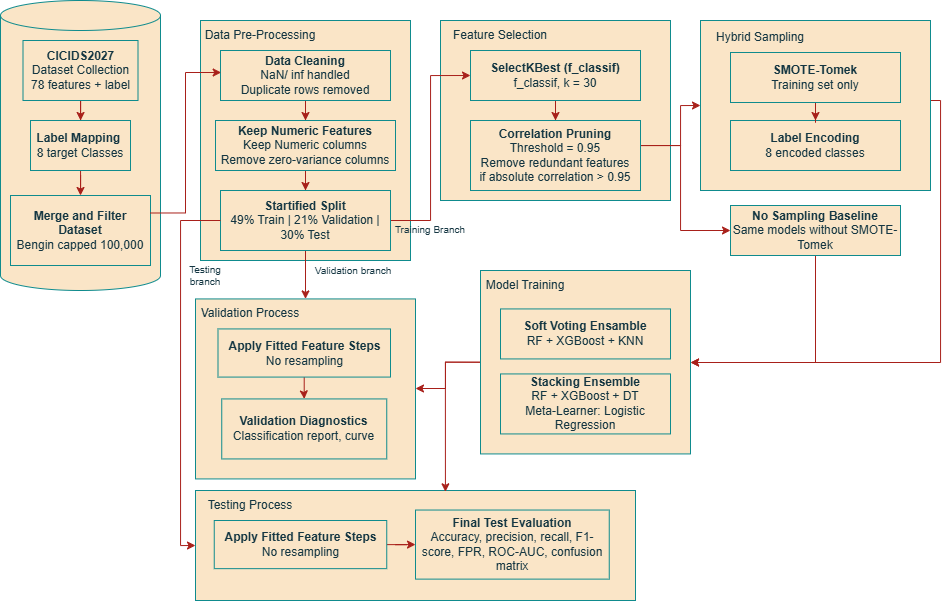
\includegraphics[width=0.95\linewidth]{Flowchart}
\caption{Overall research workflow from dataset preparation to final evaluation.}
\label{fig:method_pipeline}
\end{figure}

\subsection{Dataset}

CICIDS2017 is a public benchmark from the Canadian Institute for Cybersecurity, University of New Brunswick, containing 2,830,743 labeled bidirectional flow records with 78 features and one label \cite{khan2024balanced,nassreddine2025ensemble}. The raw labels were consolidated into eight categories: \texttt{BENIGN} to Benign; \texttt{Bot} to Bot; DoS labels, \texttt{DDoS}, and \texttt{Heartbleed} to DDoS; \texttt{PortScan} to Port Scan; \texttt{Infiltration} to Infiltrations; Patator and Web Attack-Brute Force labels to Brute Force; XSS labels to XSS; and \texttt{Sql Injection} to SQL-Injection. No labels were dropped after mapping. To reduce normal-traffic dominance while retaining attack samples, Benign was randomly limited to 100,000 records using random seed 42. The resulting class counts are shown in Table~\ref{tab:class_dist}.


\begin{table}[htbp]
\caption{Class Distribution Across Main Processing Stages}
\label{tab:class_dist}
\centering
\scriptsize
\renewcommand{\arraystretch}{1.15}
\setlength{\tabcolsep}{3pt}
\resizebox{\linewidth}{!}{%
\begin{tabular}{|l|r|r|r|}
\hline
\textbf{Label} & \textbf{Cleaned} & \textbf{Train Before} & \textbf{Train After} \\
\hline
Benign & 97,947 & 47,994 & 76,724 \\
\hline
Bot & 1,953 & 957 & 76,996 \\
\hline
Brute Force & 10,622 & 5,204 & 76,385 \\
\hline
DDoS & 321,775 & 157,669 & 157,551 \\
\hline
Infiltrations & 36 & 17 & 77,000 \\
\hline
Port Scan & 90,819 & 44,501 & 76,842 \\
\hline
SQL-Injection & 21 & 11 & 76,999 \\
\hline
XSS & 652 & 320 & 76,400 \\
\hline
\end{tabular}
}
\end{table}

\subsection{Data Preprocessing}

Data preprocessing was done to ensure data quality and model robustness for dataset CICIDS 2017. Data cleaning involved remove the redudant entries and missing values to prevent bias on parameter estimation during training. The feature set was restricted to numerical attributes, in order to optimize the input for the ensemble model. 

To preserve the original data distributions, a stratified sampling approach was used for both the initial train-test-validation (49\%/30\%/21\%) split, and followed by k-fold cross-validation. This ensures that the minority attack classes are proportionally represented, and preventing "fold-bias". Also, ensuring that the evaluation metrics accurately reflect the model's ability to detect rare intrusion events.

\subsection{Feature Selection}

ANOVA-based univariate selection (SelectKBest with \texttt{f\_classif}) was implemented to enhance model interpretability and mitigate the curse of dimensionality. This process only on the training partition to prevent data leakage, ensuring the validation and test sets remained unseen. SelectKBest with \texttt{f\_classif} was used to identify the top 30 features. This method was selected because it effectively ranks attributes by their statistical by separating discrete class labels, which is critical to identify distinct intrusion patterns. Pearson correlation pruning was used to the remaining features. By removing the redudant features if absolute correlation coefficient $|r| > 0.95$. This reduction from 70 to 16 features ensures the ensemble models focus on the most discriminative, and independent variables.


\subsection{Imbalanced Data Handling}

To determine the optimal sampling method, this research evaluated four sampling paradigms such as SMOTE, Tomek Links, SMOTE-Tomek, and the baseline no sampling, using a Decision Tree classifier. Evaluation shows that both SMOTE and SMOTE-Tomek achieved similiar overall F1-scores. While, SMOTE successfully solves the quantity problem by creating synthethic data, it sometimes creates syntetic pointes right in the middle of the majority class, which can lead overlapping. SMOTE-Tomek was selected as the sampling framework, by using Tomek links to remove those overlapping that was created by SMOTE.

\subsection{Proposed Ensemble Models}

Two ensemble models were trained. The soft voting ensemble used Random Forest, XGBoost, and KNN, combining predicted probabilities by averaging with \texttt{n\_jobs}=1. The stacking ensemble used Random Forest, XGBoost, and Decision Tree as base learners, with Logistic Regression as the meta-learner, five-fold internal cross-validation, and \texttt{n\_jobs}=1. Random Forest used 300 trees, maximum depth 20, balanced class weights, random seed 42, and \texttt{n\_jobs}=-1. XGBoost used 300 estimators, maximum depth 8, learning rate 0.05, subsample 0.8, column subsample 0.8, histogram tree method, \texttt{device=cuda}, \texttt{mlogloss}, and random seed 42. Decision Tree used maximum depth 20, balanced class weights, and random seed 42. Logistic Regression used \(C=0.5\), maximum iteration 2000, balanced class weights, random seed 42, and \texttt{n\_jobs}=-1. KNN used \(k=3\), Euclidean distance, and \texttt{n\_jobs}=-1.
These components were selected because prior NIDS studies reported strong results using tree-based learners, boosting, KNN, voting, and stacking for imbalanced intrusion detection \cite{farooqi2024enhancing,urmi2024stacked,nassreddine2025ensemble}.

\subsection{Experimental Setup}

The experiment was run in Google Colab using Python 3 and an NVIDIA L4 GPU. The notebook installed \texttt{imbalanced-learn}, \texttt{xgboost} \(\geq\) 2.0.0, \texttt{seaborn}, and \texttt{joblib} when needed, but exact package versions were not recorded. All stochastic stages used random seed 42 where supported.

\subsection{Evaluation Metrics}

The evaluation used accuracy, precision, recall, per-class F1-score, false positive rate (FPR), macro-averaged F1-score, and macro one-vs-rest ROC-AUC. In the one-vs-rest setting, each class was treated as the positive class in turn, with \(\mathrm{TP}\), \(\mathrm{TN}\), \(\mathrm{FP}\), and \(\mathrm{FN}\) denoting true positives, true negatives, false positives, and false negatives. The metrics were computed as follows:

\noindent\text1. Accuracy: Accuracy measures the proportion of correct predictions, including true positives and true negatives, to the total number of instances.
\begin{equation}
\mathrm{Accuracy} = \frac{\mathrm{TP}+\mathrm{TN}}{\mathrm{TP}+\mathrm{TN}+\mathrm{FP}+\mathrm{FN}}
\label{eq:accuracy}
\end{equation}

\noindent\text2. Precision: Precision measures the proportion of correctly predicted attacks to all samples predicted as attacks.
\begin{equation}
\mathrm{Precision} = \frac{\mathrm{TP}}{\mathrm{TP}+\mathrm{FP}}
\label{eq:precision}
\end{equation}

\noindent\text3. Recall: Recall measures the proportion of correctly predicted positive instances out of all actual positive instances.
\begin{equation}
\mathrm{Recall} = \frac{\mathrm{TP}}{\mathrm{TP}+\mathrm{FN}}
\label{eq:recall}
\end{equation}

\noindent\text4. F1-score: F1-score is the harmonic mean of precision and recall.
\begin{equation}
\mathrm{F1} = \frac{2 \times \mathrm{Precision} \times \mathrm{Recall}}{\mathrm{Precision}+\mathrm{Recall}}
\label{eq:f1}
\end{equation}

\noindent\text5. False Positive Rate: FPR measures the proportion of negative instances that are incorrectly predicted as positive.
\begin{equation}
\mathrm{FPR} = \frac{\mathrm{FP}}{\mathrm{FP}+\mathrm{TN}}
\label{eq:fpr}
\end{equation}
Because accuracy can hide weak minority-class detection, the discussion emphasizes Brute Force precision, recall, F1-score, and FPR.

\FloatBarrier

% ============================================================
\section{Results and Discussion}
% ============================================================

This section discusses the main results obtained from the experiment, focusing on the effect of class balancing, the selected flow features, and the performance of each classifier. Since the dataset was still imbalanced, the discussion does not rely only on accuracy. A high accuracy score can still be misleading when the model performs well on dominant classes but fails to detect smaller attack classes.

For this reason, the interpretation gives more attention to macro F1-score, macro recall, macro FPR, and Brute-Force-specific results. These metrics are more useful for understanding whether the proposed pipeline actually improves Brute Force detection, rather than only increasing the overall number of correct predictions. The following discussion therefore connects the validation and test results with the main objective of this study, which is to improve Brute Force detection under multiclass imbalance.

\subsection{Effect of Hybrid Sampling on Class Representation}

Table~\ref{tab:sampling_selection_macro} shows the five-fold validation results used to select the sampling strategy. SMOTE-Tomek achieved the strongest macro F1-score at 83.83\%, the highest macro precision at 83.85\%, the highest macro recall at 89.10\%, and the highest macro ROC-AUC at 94.99\%. Tomek Links produced the highest macro accuracy at 99.93\% and the lowest macro FPR at 0.0450\%, but its macro F1-score was lower than the no-sampling baseline.

\begin{table}[!htbp]
\caption{Sampling Method Selection Based on Validation Macro Performance}
\label{tab:sampling_selection_macro}
\centering
\scriptsize
\renewcommand{\arraystretch}{1.15}
\setlength{\tabcolsep}{3pt}
\resizebox{\linewidth}{!}{%
\begin{tabular}{|l|r|r|r|r|r|r|}
\hline
\textbf{Sampling Method} & \textbf{Macro Acc.} & \textbf{Macro Prec.} & \textbf{Macro Rec.} & \textbf{Macro F1} & \textbf{Macro FPR} & \textbf{Macro ROC-AUC} \\
\hline
No Sampling & 99.92\% & 80.05\% & 88.09\% & 82.02\% & 0.0484\% & 94.35\% \\
\hline
SMOTE & 99.91\% & 82.86\% & 88.41\% & 82.99\% & 0.0519\% & 94.60\% \\
\hline
SMOTE-Tomek & 99.91\% & 83.85\% & 89.10\% & 83.83\% & 0.0508\% & 94.99\% \\
\hline
Tomek & 99.93\% & 79.65\% & 86.43\% & 81.20\% & 0.0450\% & 93.42\% \\
\hline
\end{tabular}
}
\\[1ex]
\textit{Note.} Sampling strategies were evaluated with a Decision Tree classifier across five validation folds.
\end{table}

The meaning of this result is that cleaning majority-boundary samples alone can reduce false positives, but it does not necessarily improve class-balanced detection. SMOTE-Tomek was stronger because it combined synthetic minority oversampling with Tomek-link cleaning. In the final training partition, Brute Force increased from 5,204 to 76,385 samples after SMOTE-Tomek. Relative to DDoS, the largest attack class, the Brute Force imbalance changed from approximately 30.30:1 before resampling to 2.06:1 after resampling. This does not make the dataset perfectly uniform, because DDoS remained larger than the other classes, but it substantially reduced the pressure that previously made Brute Force easier to overlook during model fitting.

This finding is consistent with studies showing that hybrid sampling can improve minority-attack representation in imbalanced intrusion datasets \cite{khan2024balanced,le2024unbalanced,nassreddine2025ensemble,harini2023minority}. The selection of SMOTE-Tomek is therefore justified because it improved the most important macro-balanced indicators while also increasing the Brute Force training representation substantially. The implication is that resampling should not be judged only by overall accuracy, because the accuracy differences among sampling methods were very small. Consequently, SMOTE-Tomek became the most appropriate sampling method for this pipeline because it gave Brute Force traffic a more meaningful role in model learning without discarding the multiclass structure of the dataset.

The comparison also shows why a hybrid method is preferable to using only one balancing mechanism. SMOTE improved macro F1-score compared with no sampling, but SMOTE-Tomek produced a further improvement while also achieving the strongest macro ROC-AUC among the sampling candidates. Tomek Links alone produced the lowest macro FPR, but its lower macro recall and macro F1-score indicate that cleaning without increasing minority exposure was not sufficient for the target problem. The consequence is that the sampling choice should be interpreted as a balance between representation and boundary control. For Brute Force detection, increasing representation is essential because the original training data contain far fewer Brute Force samples than DDoS samples.

The result also explains why the final discussion does not treat every minority class as equally improved. SMOTE-Tomek created a much larger training representation for rare classes, but the quality of synthetic expansion still depends on the information available in the original samples. Brute Force had enough original support to benefit from resampling more reliably than SQL-Injection or Infiltrations. Therefore, the sampling result supports the main objective of improving Brute Force detection, while also showing that extremely small classes require more cautious interpretation.

\subsection{Selected Flow Features and Detection Meaning}

The feature-selection process reduced the original numerical feature space to 16 final features through ANOVA-based \textit{SelectKBest} and correlation pruning. Permutation-importance diagnostics showed that Destination Port was the most influential feature. The remaining high-ranked features were grouped into four flow-behavior categories: TCP window behavior, timing behavior, packet behavior, and TCP flag behavior.

These features show patterns that make sense for catching Brute Force attacks. These features capture the critical network characteristics such as the TCP initial window behavior, arrival timing, connection duration, variation of size of the packet, traffic rate and TCP flag behavior. The specific habits earned from brute force attacks are they keep attacking the same service, repeatedly, and regularly, so the useful indicators are destination service information, timing, length of the packet, and TCP-state.

The result supports claim of previous NIDS studies to use feature selection in order to address the redudant flow attributes before classification \cite{nassreddine2025ensemble,alsaffar2024shielding}. Also, supports the claim of the studies that treat Brute Force and web attacks as behavior-driven detection problems rather than just as volume-drive anomalies \cite{rihan2023iot,irfaissurur2025web}. The selected features was used because they are not only statistically important, but also meaningful in terms of how Brute Force traffic appears in network flows. This also means that the model did not only guess based on hidden math, but also it used network data that actually make sense for human. As the consequent, the result also shows the pratical credibility of the pipeline for CICIDS 2017 Brute Force attack detection, but do the validation is still required for the same important patterns that appear in different datasets before make a claim that this model works well on everything.

This explanation is important because feature importance alone can lead to misleading if the selected features do not have clear behavioral connection with the target. In this study, chosen Destination Port as the most important feature, which can be make sense because Brute Force attacks have certain behavior like always target the specific services. Features like duration and timing are also chosen as the important features, because a bot usually attacking a system that looks different. Packet-length and rate features also show additional evidence about the communication is executed when the connection was initiated. As the consequence, this selected features support both performance and interpretability. 

\subsection{Final Interpretation}

The result is based on the proposed pipeline that used to improve Brute Force detection by using the combination of SMOTE-Tomek, feature selection, and the Stacking and Soft Voting Ensemble learning. SMOTE-Tomek is used to address the issue of imbalance dataset. Feature selection is used to determine which are the features that actually relevant with the label, and also to reduced the redudant features. While Stacking and Soft Voting ensemble learning is used to make a strong prediction model. This finding is consistent with the previous Network Intrusion Detection System (NIDS) studies that highlight techniques such as hybrid sampling, feature selection, and ensemble learning \cite{khan2024balanced,nassreddine2025ensemble,alsaffar2024shielding,farooqi2024enhancing,urmi2024stacked}. When all techniques is combined it will address some issue like imbalanced dataset, limited minority samples, redudant features, and the reliance on a single classifier. 

However, the pipeline did not perform equally well across all minority classes. The final model produced strong results for Brute Force, Benign, DDoS, Bot, and Port Scan traffic, but it is performance was less stable for classes with very few test samples. SQL-Injection achieved 61.54\% F1-score from six test samples, XSS achieved 51.52\% F1-score with low precision, and Infiltrations achieved 90.00\% F1-score from only 11 test samples.  This indicates that SMOTE-Tomek was more effective for Brute Force than for classes with extremely limited original data. Therefore, although the pipeline performed well on CICIDS2017, further testing on newer datasets and more diverse traffic is still needed.

Overall, this proposed method should be interpreted as a targeted improvement for Brute Force detection, rather than the proposed solution that works well on all rare attack. Resampling can increase training representation, but it cannot replace the real traffic variety fully because the original samples are also very limited. The final model selection also reflexts this consideration. Although XGBoost and Soft Voting achieved similiar ROC-AUC values, but the stacking ensemble provided the highest macro F1-score and better false-positive control. In an imbalanced dataset in Network Intrusion Detection System (NIDS), this trade off is important because the model must be able to detect attacks effectively.

% ============================================================
\section{Conclusion and Future Research}
% ============================================================

This research proposed an enhancement for Brute Force Attack Detection in a multiclass Network Intrusion Detection System (NIDS) using the CICIDS2017 dataset. The workflow pipeline combined such as label consolidation, Benign class filtering, train-only feature selection, SMOTE-Tomek Hybrid sampling, and ensemble learning. The main aim of this research was to evaluate if this multi-stage approach could enhance detection accuracy in imbalanced environments without violate the experimental integrity through data leakage. The results show that the pipeline was effective because each component addressed a different part of the problem: feature selection reduced redundant flow attributes, SMOTE-Tomek improved minority-class representation, and the stacking model combined complementary classifiers to strengthen the final prediction.

Through the application of SMOTE-Tomek, it successfully expanded the training set for Brute Force attacks from 5,204 to 76,385 samples. This significant increase effectively managed the imbalance ratio of DDoS traffic from approximately 30 samples for every one attack to just over two samples for every one attack. Among all tested sampling techniques, SMOTE-Tomek consistently delivered the highest superior results across macro-level metrics, including F1-score, precision, recall, and ROC-AUC. As the consequent, the Stacking Ensemble combined with SMOTE-Tomek was finalized as the primary model. It not only secured the highest validation macro F1-score but also give the demonstration about best perfomance in maintaining a low macro False Positive Rate (FPR).

On the unseen test set, the final configuration achieved 99.93\% macro accuracy, 86.10\% macro precision, 90.22\% macro recall, 86.93\% macro F1-score, and 97.98\% macro ROC-AUC. For Brute Force traffic, it achieved 98.70\% precision, 92.66\% recall, 95.58\% F1-score, and 0.0253\% FPR. These results show that hybrid sampling and Ensemble Learning like Stacking and Soft Voting can improve Brute Force detection when it was applied in the vurnable leakage aware workflow. Compared with previous CICIDS2017 studies that using such as conventional classifier with SMOTE-Tomek, this research provides stronger configuration for Brute Force focused with evidence, even though the result needs to interpreted carefully because the evaluation protocols may be different.

Despite the positive results, several limitations are still consideration. First, this study relied only on the CICIDS2017 dataset, so this may not fully apply to the more modern or various network enviroments, this is a persistent challenge in machine learning based for Network Intrusion Detection System (NIDS) research \cite{sarhan2021standard,wardana2024collaborative,gu2025semisupervised}. Second, while SMOTE-Tomek significantly optimized the Brute Force target, its impact was less consistent on extremely minority classes. As the evidences in the performance for example SQL-injection which contains only 6 test samples, and XSS which has low precision, and Infiltrations which consist only 11 test samples. Third, the use of synthetic resampling may have introduced bias, especially where original class data was severely minority. Fourth, specific library version and the Google Colab runtime were not documented or written, which can effect the exact reproducibility. Fifth, during the validation phase, the absence of feature scaling or normalization may have effected the performance of distance-sensitive models, such as KNN and Logistic Regression.

Future research is suggested to test the pipeline on additional datasets and more newest traffic environments to notice whether the selected features and classifier behavior remain stable outside the CICIDS2017 dataset. Futher studies are also hoped to record exact dependency versions, evaluate train only feature scaling for sensitive scale model and compare the porposed workflow with other ensemble configurations under the same vurnable leakage aware protocol. For extermely minority classes, future work should explore additional real attack samples, recent sampling methods, or few shot learning to reduce dependence on synthetic data.

Overall, this study shows that improving minority-attack detection requires more than simply adding resampling to a classifier. The strongest result was achieved when class representation, feature relevance, and model diversity were handled together in one workflow. In practice, Brute Force detection should be evaluated by considering both missed attacks and false alarms. High recall helps reduce undetected attack attempts, while high precision and low FPR help maintain trust in NIDS alerts. Therefore, the contribution of this study lies not only in the final performance score, but also in showing that each stage of the pipeline supports the Brute Force detection objective.


\FloatBarrier

% ============================================================
\section*{Open Data}
% ============================================================

The CICIDS-2017 dataset is publicly available via the CIC repository and can be obtained from the following website: 
\url{https://www.unb.ca/cic/datasets/ids-2017.html}.

The source code used in this study is publicly available via Github and can be obtained from the following website:
\url{https://github.com/jetasunanda/Enhancing_Brute_Force_Attack_Detection}.

% ============================================================
\section*{Author Contributions}
% ============================================================

\textbf{Edward Aria Tanujaya:} Introduction, Result and Discussion, Conclusion, Writting - review \& editing. \textbf{Jeta Sunanda:} Related Works, Result and Discussion, Conclusion, Writting - review \& editing. \textbf{Andrian Pratama:} Methodology, Resources, Writting - review \& editing, Result and Discussion. \textbf{Hidayaturrahman:} Validation, Supervision. \textbf{Satriadi Putra Santika:} Validation, Supervision.
 
% ============================================================
\bibliographystyle{IEEEtran}
\bibliography{references}

\end{document}
